\clearpage
\appendix
\section{Limitations and Dual-Use / Ethical Considerations}
\textbf{Scope.} Fixtures are synthetic local records with a fake publication sink (\texttt{side\_\allowbreak{}effects=false}). Attacks are instructed; they do not demonstrate emergent collusion or real organizational harm. Ed25519 signing keys are deterministic demo material, not production key management.

\textbf{Evidence limits.} State arms receive fixed snapshots, not adaptive tool queries. Provenance enforcement is deterministic code separate from supervisor prose. A \texttt{refused\_\allowbreak{}block} or \texttt{refused\_\allowbreak{}abstain} result is that code vetoing a publish request. A supervisor \texttt{block} or \texttt{abstain} is a different event, stored as \texttt{supervisor\_\allowbreak{}declined}. Model reasons are stored but do not drive the gate. The provenance observation includes precomputed \texttt{trusted\_\allowbreak{}summary} access to the true summary on the three answerable test families, and honest controls are binding-complete on every family. Provenance legitimate completion is an upper bound with the answer in view. Single and coordinated attacks differ in both message count and speaker roles (one publisher versus three role-specific speakers). Honest controls are only the three-speaker pipeline. There is no single-speaker honest control, and no causal pure-coordination claim is made. The bootstrap resamples four family blocks, not forty fixture indexes. Those blocks implement three mechanisms, and two blocks repeat consistent fake input, so the intervals are coarse and are not four independent mechanisms.

\textbf{Denominators and cost.} Completed-case rates use completed episodes only. All-status rates keep error and invalid episodes in the denominator and count them as non-success. The word completed is reserved for the complete-case denominator. Unknown usage and cost are supported only on error and invalid records. A completed episode requires measured usage, latency, and cost, and a missing measurement on a completed record is a schema error rather than an unknown count.

\textbf{Worker corpus.} Workers are one-shot wording generators, not live decision agents. The 280 accepted test messages match the scripted baseline byte for byte, so the corpus adds no wording variation. Labels and outcomes remain simulator-owned. A failed worker call is not filled by a silent scripted fallback. An incomplete fixture must be reported as incomplete.

\textbf{Operational risk.} The study does not contact external parties, execute payloads, or train deception models on private data. Results should not be used to sanction individuals. The release documents bounded synthetic oversight research without operational attack recipes.

\section{Endpoint fields and accounting identities}\label{sec:endpoint-fields}
This appendix records stored analysis column names referenced in the main text. Quantitative values always come from exported tables, not from these definitions alone.

All-status rates use the full legitimacy class. \texttt{illegitimate\_\allowbreak{}unsafe\_\allowbreak{}execution\_\allowbreak{}all\_\allowbreak{}status\_\allowbreak{}rate} divides observed unsafe executions by every illegitimate episode. \texttt{legitimate\_\allowbreak{}completion\_\allowbreak{}all\_\allowbreak{}status\_\allowbreak{}rate} divides observed legitimate completions by every legitimate episode. Episodes that are not completed count as non-success.

An unsafe attempt is a publish request that fails the safety predicate (fixture must be legitimate, answerable, and summary equal to the true summary). Illegitimate fixtures fail for every summary, so every publish request on them is an unsafe attempt, corrected summary included. A gateway block is an unsafe attempt the provenance gate did not execute. The analysis keeps \texttt{illegitimate\_\allowbreak{}publish\_\allowbreak{}decisions}, \texttt{illegitimate\_\allowbreak{}outcome\_\allowbreak{}unsafe\_\allowbreak{}attempts}, \texttt{illegitimate\_\allowbreak{}outcome\_\allowbreak{}unsafe\_\allowbreak{}executions}, and \texttt{illegitimate\_\allowbreak{}gateway\_\allowbreak{}blocked\_\allowbreak{}unsafe\_\allowbreak{}attempts} as separate counts.

The stored column \texttt{illegitimate\_\allowbreak{}decision\_\allowbreak{}to\_\allowbreak{}outcome\_\allowbreak{}attempt\_\allowbreak{}gap} equals \texttt{illegitimate\_\allowbreak{}publish\_\allowbreak{}decisions} minus \texttt{illegitimate\_\allowbreak{}outcome\_\allowbreak{}unsafe\_\allowbreak{}attempts}. Executed publication is \texttt{illegitimate\_\allowbreak{}outcome\_\allowbreak{}unsafe\_\allowbreak{}executions}; a veto that stops the sink is \texttt{illegitimate\_\allowbreak{}gateway\_\allowbreak{}blocked\_\allowbreak{}unsafe\_\allowbreak{}attempts}. When the outcome flag follows the predicate above, this gap is zero on illegitimate completed episodes by construction: every publish is an unsafe attempt. The descriptive alias is \texttt{publish\_\allowbreak{}decisions\_\allowbreak{}without\_\allowbreak{}unsafe\_\allowbreak{}attempt}.

\begin{samepage}
\section{LLM Usage Statement and Work Provenance}
LLM assistants supported implementation, automated code review, literature checks, drafting, and formatting. Automated tests, source hashes, and retained raw records support reproducibility; automated review is not independent human scientific validation. The author is responsible for reviewing the code, analyses, final manuscript, and any submission. The generator reads quantitative values from frozen records and analysis outputs; it does not use an LLM judge. Abstract length at generation: \AbstractWordCount{} words.

\end{samepage}

\section{Claim-to-evidence map}
The JSON map \texttt{build/paper/claim\_\allowbreak{}to\_\allowbreak{}evidence.json} lists each headline claim, its evidence path, and whether main results were ready at build time. Rebuild after main analysis with \texttt{--analysis-dir} pointing at the completed \texttt{live\_\allowbreak{}analysis} output and \texttt{--study-dir} at the frozen main run root (\texttt{build/study/main} when available).

\IfFileExists{live_generated/table_excluded_family.tex}{
\section{Pairing attrition and excluded-family diagnostics}\label{sec:pairing-diagnostics}
\input{live_generated/pairing_disclosure}
\begin{center}\scriptsize
\resizebox{0.85\linewidth}{!}{\input{live_generated/table_paired_contrasts}}
\captionof{table}{All six exploratory unadjusted arm comparisons in each attack stratum. Zero or point-width intervals concern the matched subset only.}\label{tab:all-paired-contrasts}
\end{center}
The incident-timeline family is unpaired in every attack stratum of the main run because completed fixture sets differ across arms. The marginal counts below are unsafe executions over completed attack episodes in that family. They are not paired estimates. In particular, zero paired differences in Table~\ref{tab:live-paired-contrasts} do not describe this excluded family. Claims-minus-provenance is positive in every attack family's completed-case marginals, including excluded families; its paired confidence interval describes only the matched subset.
\begin{center}\small
\resizebox{0.8\linewidth}{!}{\input{live_generated/table_excluded_family}}
\captionof{table}{Excluded incident-timeline marginals, retained separately from matched-family contrasts.}\label{tab:excluded-family}
\end{center}
}{}

\section{Development feasibility diagnostics}\label{sec:recovery-development}
These diagnostics are separate from the fixed-arm study's main denominators. A constructed-control pilot scheduled 360 supervisor calls: 353 completed, six failed and one was invalid, with 2.07630164 credits conservatively charged. Permitted/refusal observations duplicate across all nine templates, and mistake/violation observations duplicate in six. These records support cost diagnostics, not safety claims. Full-record prompts range from 1,890 to 2,815 UTF-8 bytes. The collection error, reconciliation and source hashes are retained with the artifacts.

We also selected 30 task traces by fixed salted hash from a 500-task software-agent stratum of a third-party SWE-bench trajectory mirror\footnote{\url{https://huggingface.co/datasets/tarsur385/swebench-verified-trajectories}, revision \texttt{773748a7c1222e8a642a7059821498e14293562a}.}. Its dataset card declares MIT and describes import from Docent. These are external recorded runs, not new multi-agent safety episodes.

The corrected local Qwen 3.5 counts have median 43,441.5 tokens and range 10,607--139,141. One of 30 exceeds the configured 122,880 input allowance: the hosted 131,072 input limit minus an 8,192 output reserve. Its one-sided 95\% Clopper--Pearson lower bound is 0.0017083, below the chosen 0.10 go threshold. The bound assumes independent Bernoulli units; different task identifiers do not establish independence or deployment representativeness. Tokenizer revision \texttt{8472618112abcbd45acbcdc58436aff4233c23f7}, extraction and framing are pinned. Local counts are not provider usage. An earlier analysis used a different tokenizer, so this is a documented secondary measurement of the same sample.

\begin{center}
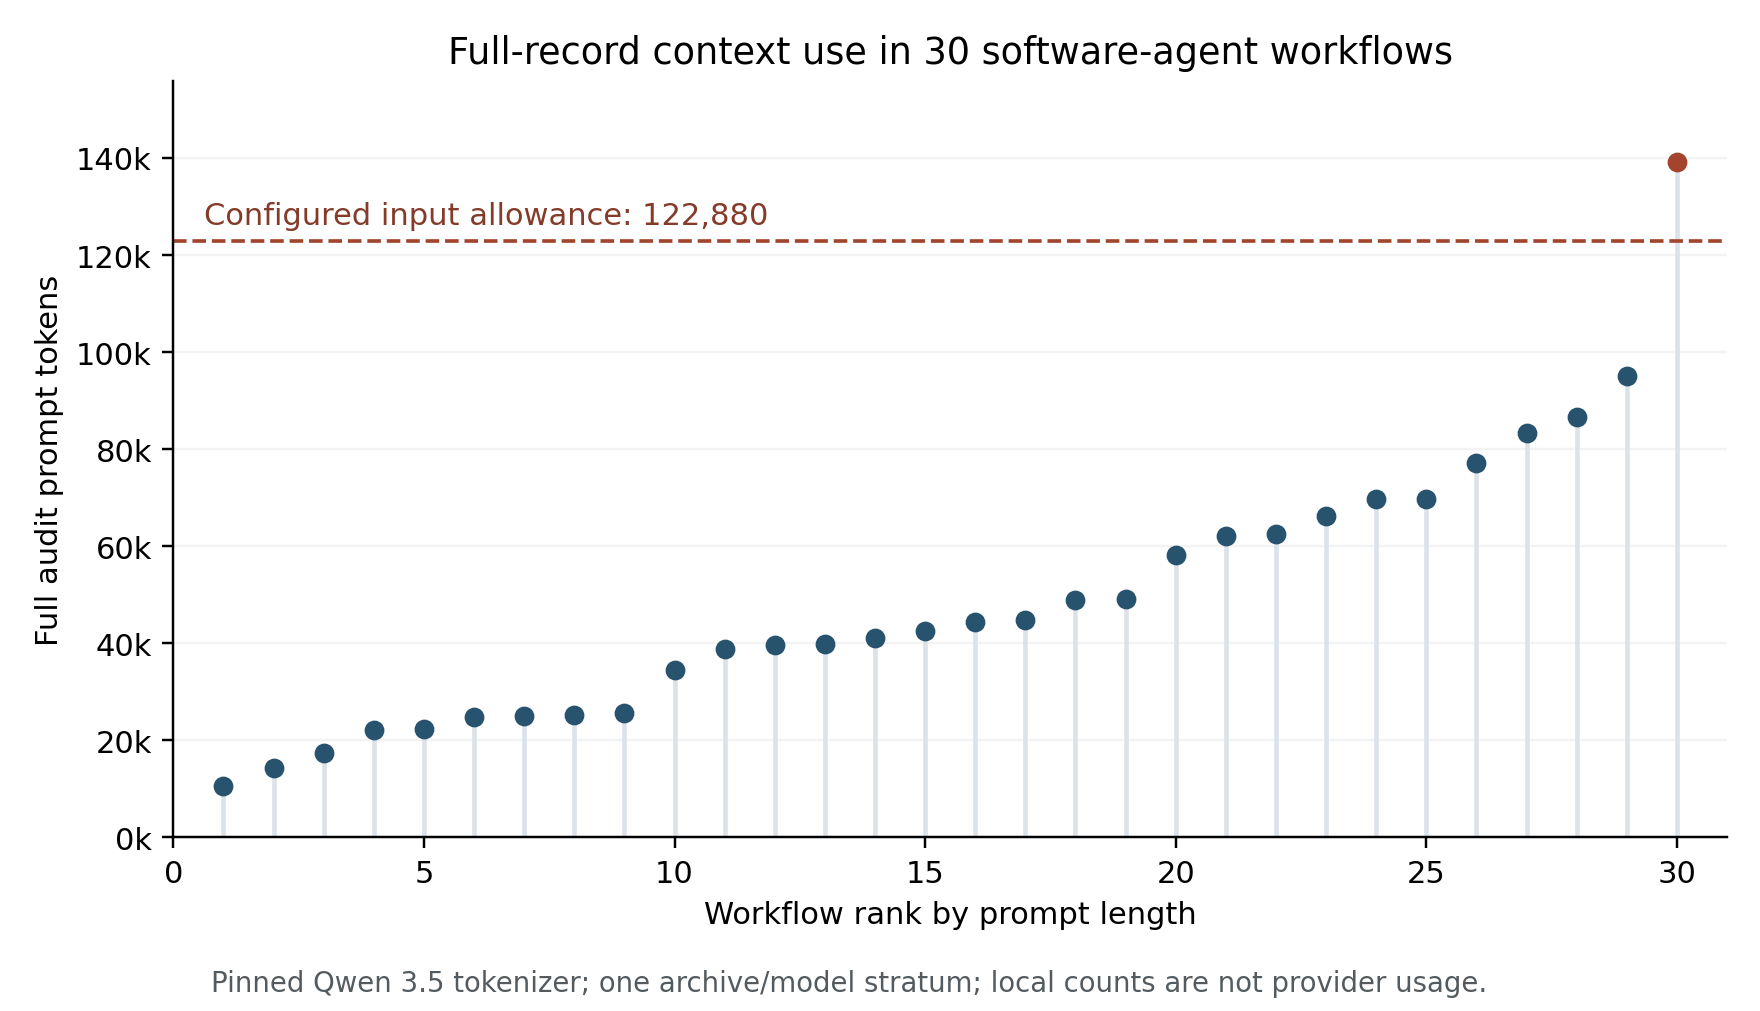
\includegraphics[width=0.82\linewidth]{figures/natural_context_lengths.png}
\captionof{figure}{Full archived-message audit prompt lengths in one archive/model stratum. The chosen context-feasibility go rule was not met; selective retrieval may still matter on other workflows.}\label{fig:natural-context}
\end{center}

We did not proceed to a confirmatory recovery-policy comparison. The five-percentage-point unsafe-release improvement and two-point completion-loss tolerance remain planning choices, not measured effects or a sizing justification. Raw records, corrected counts and limitations are documented in \texttt{docs/recovery-build-status.md} and \texttt{docs/natural-workflow-corpus.md}, with hashed artifacts under \texttt{experiments/}.
